\ignore{
\begin{verbatim}
 * Overview
    High-level exec. semantics
    Coverage wrt threat model
 * Detailed (micro)architecture
    * Buffers
    * ISA extensions
 * Putting it all together
    [Flowcharts?]
    * Behavior under speculation
    * Behavior under non-speculative exec.
    * Relation to value prediction
* Overheads?
* Correctness guarantee?
* New vulnerabilities?
 \end{verbatim}
 }
 
 \begin{figure*}
     \centering
     \subfloat[Slice example]{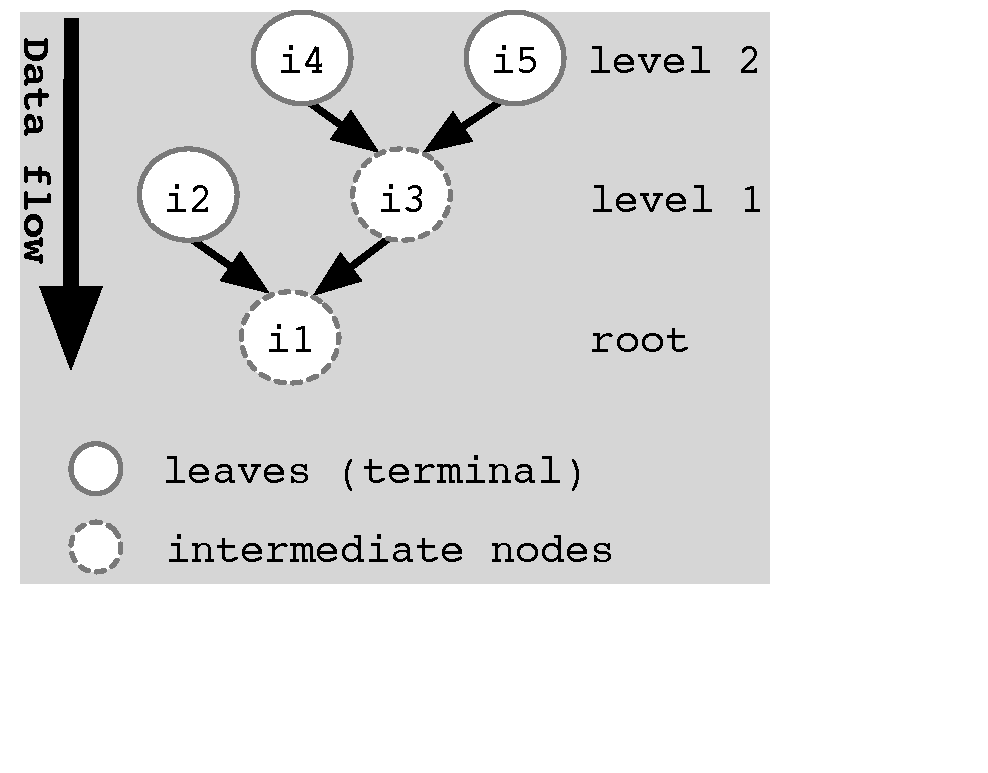
\includegraphics[width=0.3\textwidth]{figs/rt.pdf}\label{fig:rt}}
     ~~~
     \subfloat[Execution semantics and  $\mu$-architecture]{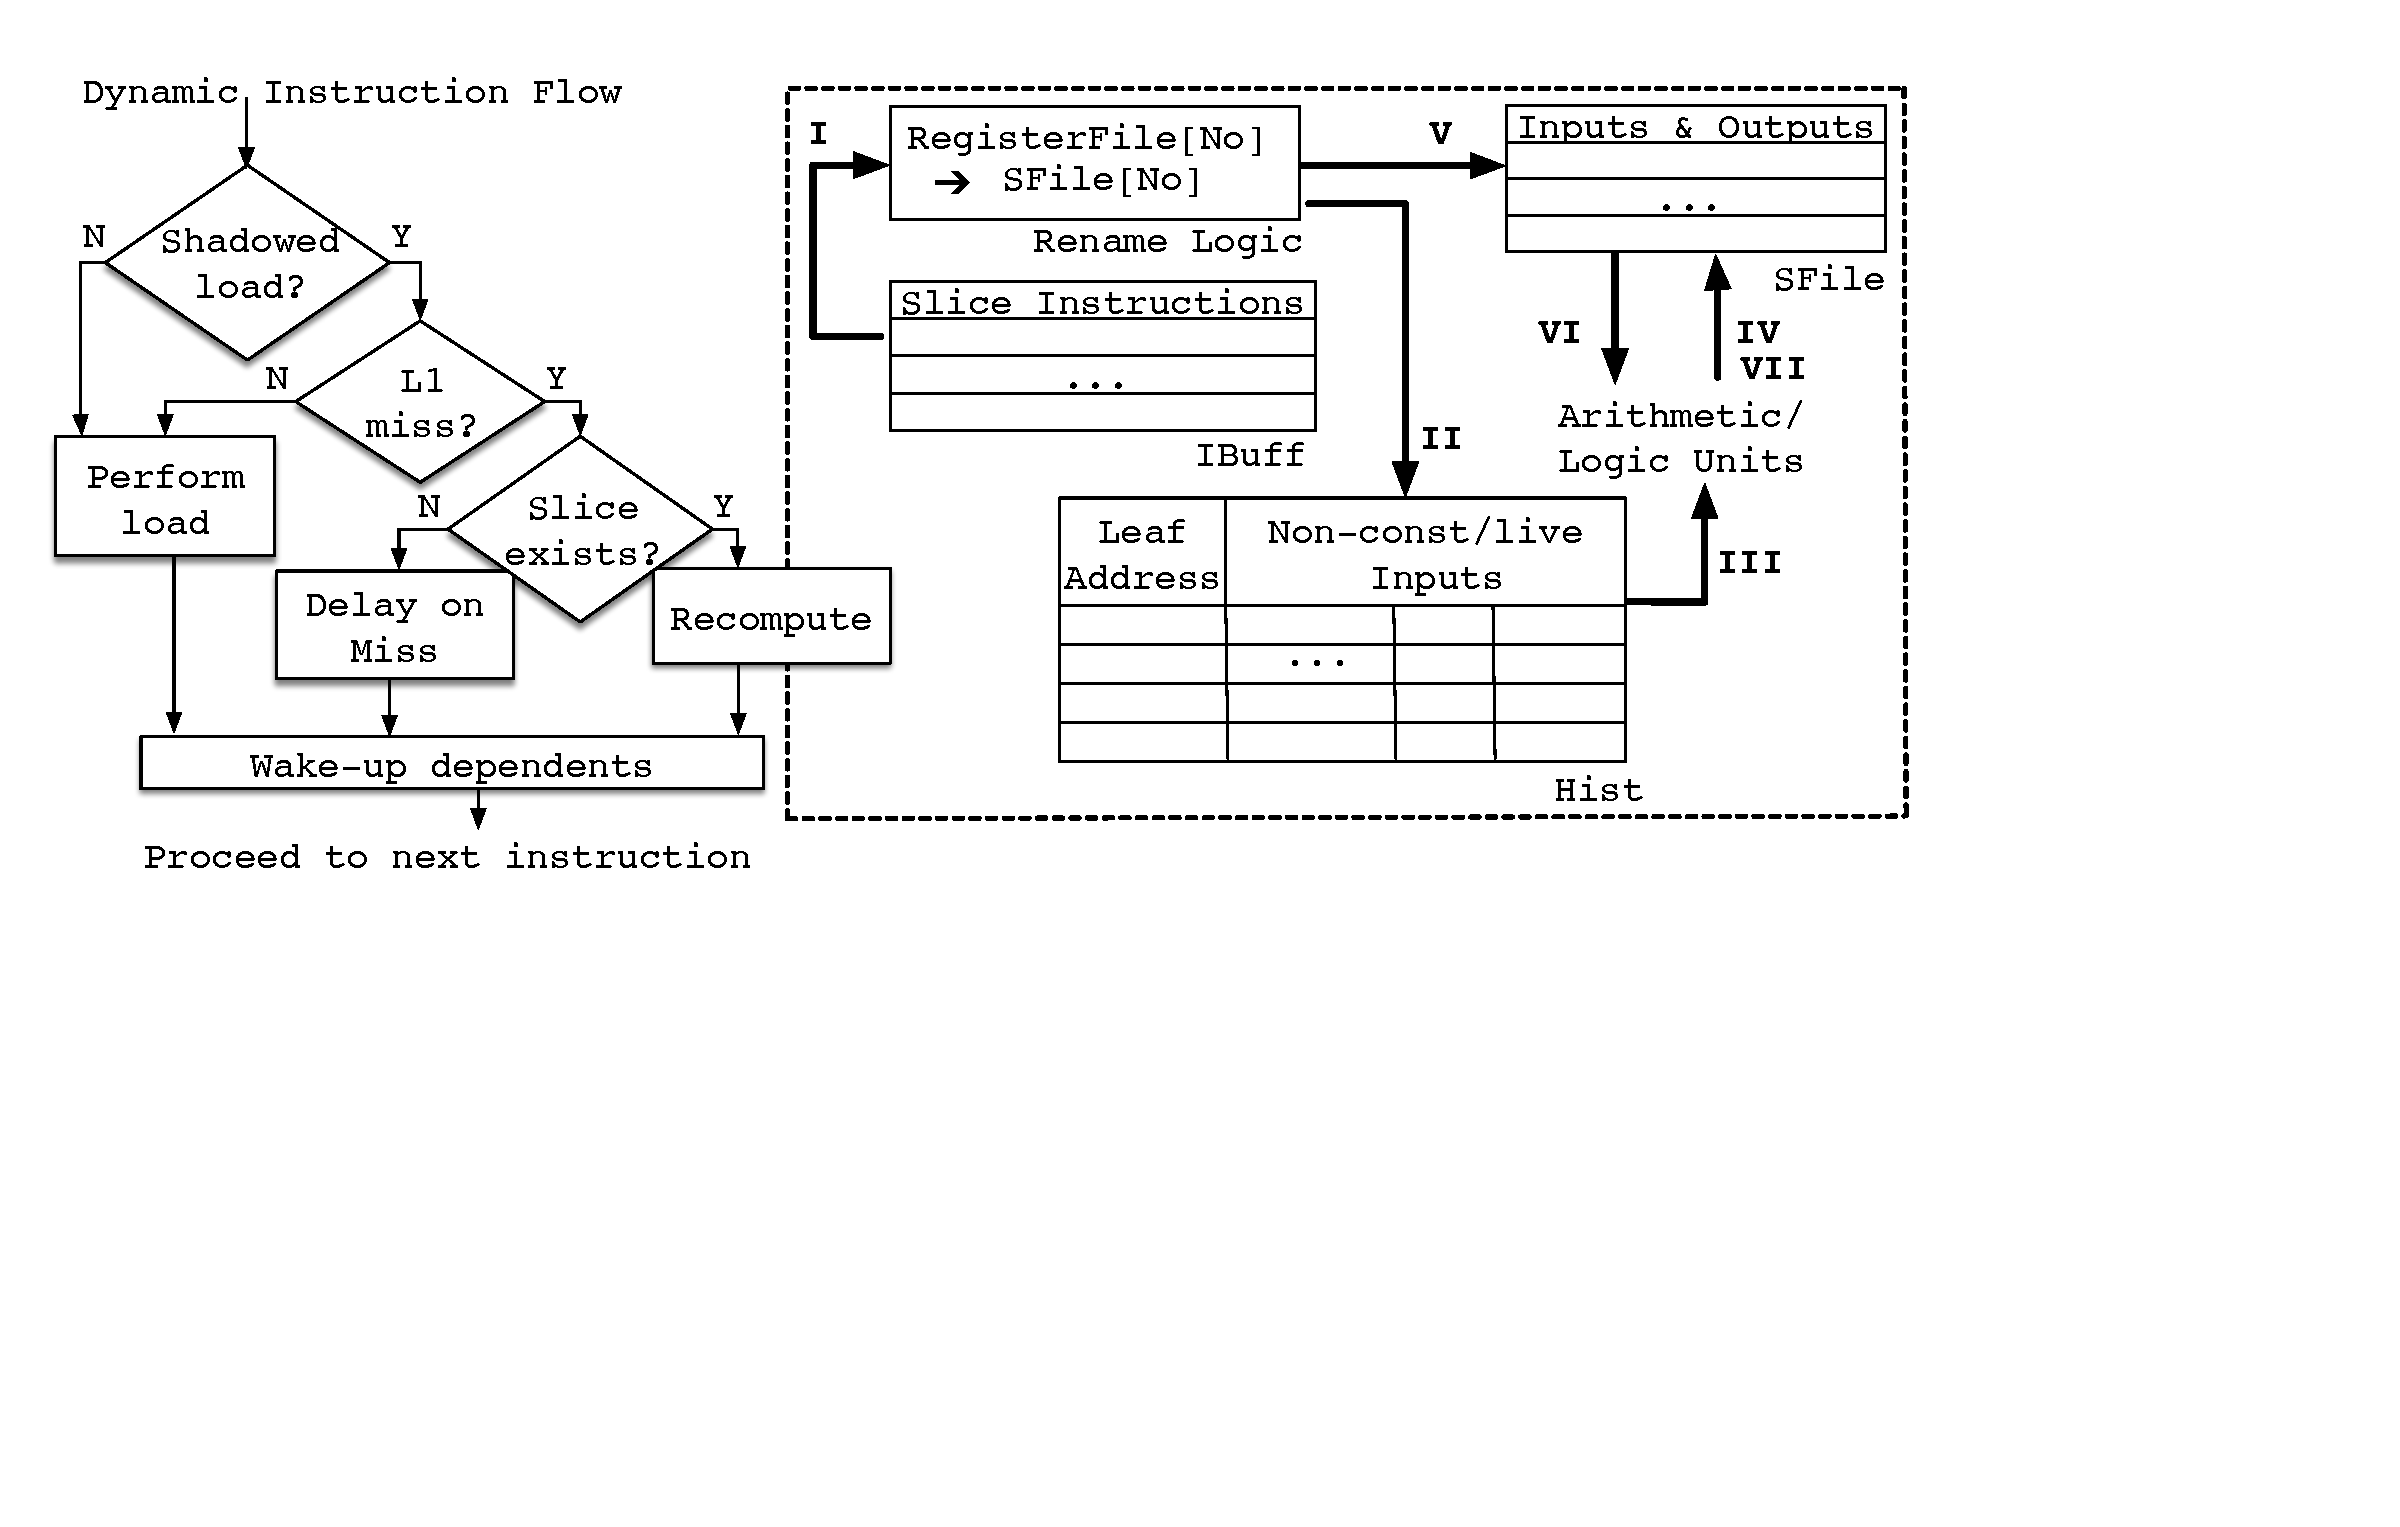
\includegraphics[width=0.57\textwidth]{figs/ctrl.pdf}\label{fig:ctrl}}
     \caption{ \arch\ Overview. All $\mu$-architectural buffers from (b) have  
an $\texttt{invalid}$ field per entry to
manage space (de)allocation.}
     \label{fig:overview}
\vshrink{.2}
\end{figure*}
 
% Overview
 
 \subsection{Execution Semantics}
 
 \arch{} only resorts to recomputation to regenerate values that otherwise would be read by a speculative load from the memory hierarchy, and only so, if the respective speculative load misses in the L1 cache. Recomputation takes place as long as a slice exists and the input operands to the slice instructions can be made readily available (see \autoref{sec:slice_formation} on slice formation).
 %This execution model has the potential of delivering higher energy efficiency, as imbalanced technology scaling renders loads much more energy hungry and slower than arithmetic/logic instructions (which form slices)~\cite{Horow}. 
 %Typically a slice contains \redHL{no more than 10-15 instructions}.
 
\ignore{
Not all of the input operands of leaf instructions of a slice can be
(re)generated by recomputation.  This may be the case if input operands
correspond to (i)~read-only values to be loaded from memory, such as program
inputs; or (ii)~register values that are lost, i.e., overwritten at the time of
recomputation. We will refer to such input operands as {\em non-recomputable}
inputs. For \recomp\ to work, non-recomputable inputs of slice-leaves
should not only be available at the anticipated time of recomputation, but also
be retrievable in an energy-efficient manner.
%
%Recomputation cannot eliminate any memory access to retrieve the non-recomputable inputs of slice leaves.  
If non-recomputable inputs do not
reside in close physical proximity to the processor, the energy cost of their
retrieval may easily exceed the energy cost of memory accesses, rendering recomputation useless.    
Buffering can help in this case. No dedicated buffering is necessary if the leaf input operands
correspond to constants or live register values. 
}

While \arch\ shares basic microrachitectural structures with Amnesiac~\cite{amnesiac17} to facilitate \recomp\ (such as dedicated buffers to prevent corruption of $\mu$-architectural state during recomputation), its
execution semantics are quite different when it comes to slice identification and triggering recomputation.
%, and committing recomputed values to architectural state. 
These stem from the defining difference in optimization targets: Amnesiac uses \recomp\ to maximize energy efficiency irrespective of security implications. \arch, on the other hand, uses \recomp\ to eliminate (already known or yet to be discovered) threats induced by speculative loads. 
In a nutshell, differences between Amnesiac and \arch\ expand along two axes:
%Putting it all together, execution semantics are different than Amnesiac~\cite{amnesiac17} in the following ways:
 \begin{itemize}
     \item{\em What to recompute (slice identification):} As opposed to Amnesiac, \arch\ does not impose any direct constraint 
     %on slice length 
     to preserve energy efficiency,  as we are not after minimizing energy or latency per load. As long as a slice exists, and its inputs can be made readily available at the anticipated time of recomputation, \arch\ would consider it for recomputation. The only practical limitation on slice length may stem from storage overhead of $\mu$-architectural buffers in this case. 
     \item {\em When to recompute:} \arch\ swaps speculative loads that miss in L1 for recomputation (i.e., with producer instructions of the respective value along a slice). Amnesiac on the other hand, triggers recomputation (irrespective of whether the load is speculative or not) only if it is more energy-efficient to do so. 
 %    \item{\em How to recompute?} Similar to Amnesiac, we use dedicated buffers to prevent corruption of $\mu$-architectural state. 
     \ignore{
     \item{\em When/how to commit a recomputed value to architectural state:}
     \textcolor{blue}{\\ HMS: {\recomp} is non-speculative and safe, they don't have to adhere to the shadows. It's the action of the load itself that has to be avoided, which it is, so the {\recomp} computed value can be treated as any other transient register, e.g., the result of an addition. Thus, I don't see any difference compared to Amnesiac. 
     U: Noted, and elimiated\\}
     In Amnesiac, a recomputed value is written into the destination register of the  load before execution resumes from where the corresponding load (which is swapped for recomputing instructions) has left. 
     \arch\ has to keep these values buffered until the speculation is resolved (i.e., all shadows are lifted).  
     \recomp\ cannot change architectural state under speculation, by definition. {However, just as speculative loads that \emph{hit} in the L1, recomputed loads pass their value (in a physical register) to dependent instructions and advance execution.} }
 \end{itemize}
 
 In the following sections, we will cover design specifics, limitations, and side effects of \arch, with a special focus on coherence and consistency implications. 
 
% We will detail design specifics next. 
 
\subsection{Slice Formation \& Annotation}
\label{sec:slice_formation}

%\noindent{\bf Slice Formation:}
Similar to Amnesiac, we rely on a compiler pass (backed up by profiling) to form and annotate slices, which 
 mainly constitutes
%first estimates,
%probabilistically 
%(as detailed in the following and Section~\ref{sec:setup}),
%\footnote{Section~\ref{sec:setup} details a representative
%probabilistic model based on memory access statistics collected from profiling.}
%the energy
%consumption of loading $v$, $E_{ld,v}$. Next comes 
%with 
dependency analysis to
identify the producer instructions for each load.\footnote{Instead of a compiler,
%, in order to calculate the anticipated
%cost of potential recomputation.
%\textcolor{blue}{HMS: I think this idea is currently too immature to be included.}
%\redHL{U: Our implementation is actually Pin-based, if this is what you were referring to?}
%\textcolor{blue}{HMS: I might have misunderstod the text. I was reading the following text as it could be done at runtime while executing the application (in deployment every time the application is run), not as a "profiling pass".}
%\redHL{Yes, this may open Pandora's box, need to clarify.}
%{\color{magenta}  
the same job can be performed by \emph{dynamic binary instrumentation} at run time (albeit with probably inferior alias analysis but more dynamic information), rendering recompilation unnecessary in deployments where it is not an option.}
Slice creation is a \emph{best effort} under strict validity guarantees. Not being able to generate a recomputation slice for a load is not a security weakness under a security technique such as Delay-on-Miss, but simply a missed optimization opportunity.
 Although in this paper the slice formation is conservative, as we will see later, the requirement for strict guarantees of the recomputation validity can be relaxed (potentially increasing the coverage of recomputation, i.e., portion of load values that can be recomputed, and addressing coherence issues) if the appropriate architectural support is available. However, such extensions are outside the scope of this paper and will be fully evaluated in future work.
%}

The slice formation pass builds the slice as a data-dependency graph, where
%%This step starts building the slice (where 
the immediate producer of the value to be loaded resides at the root (Figure~\ref{fig:rt}).
%%), and lets the slice grow
%%level by level. 
As opposed to Amnesiac, the restriction to slice length comes from slice inputs or storage requirements (rather than the associated energy cost). 
%, as long as the cumulative cost of recomputation along \rsv\
%being constructed remains below $E_{ld,v}$.     
If, during the traversal of data dependencies, we encounter other load instructions, we 
%As the compiler traverses the dependency chains, it may hit
%load instructions. In the proof-of-concept implementation, the
%compiler replaces each such load 
replace them recursively with the respective producer instructions. 
%recursively.
This recursive growth can continue until a store to the same address is encountered.
Loads and stores cannot be present 
%as intermediate nodes 
in any slice by definition.
%In fact, stores can never find place in \rsv, and loads can only, if at all,
%appear at the leaves to read non-recomputable input operands.

Once construction is complete, 
%corresponding 
each slice gets embedded into the binary. 
Similar to Amnesiac, the special control
flow instruction $\texttt{RCMP}$ communicates recomputation opportunities to the runtime, which
%we use 
%\noindent {\bf Slice Annotation:}
%\label{sec:isa}
%As a hint for the runtime scheduler, the compiler replaces each load that has a slice
%the swap
%of which with recomputation is likely to be more energy-efficient (according to
%the probabilistic energy cost comparison explained above) 
%with a 
semantically corresponds to an atomic bundle of a conditional branch + load (where no prediction is involved for the ``branch'' portion).
%In this manner, the recomputing instance of an
%instruction is separated from its original, ``computing'' instance.
%Semantically, $\texttt{RCMP}$ corresponds to the fusion of a conditional branch
%with a load\footnote{
%Depending on the specifics of the underlying instruction set architecture (ISA),
%$\texttt{RCMP}$ can also be synthesized by a pair of branch and load
%instructions, without loss of generality. 
%}. 
The runtime scheduler resolves the branching condition: if the respective load (while shadowed) misses in L1, $\texttt{RCMP}$ acts as a jump to the entry point (starting from the
terminal instructions) of the corresponding slice. Otherwise (i.e., if the load hits in L1 when shadowed or if the load is not shadowed), $\texttt{RCMP}$ acts as %is not any different than 
a classic load.
All operands of the respective load and the starting address of its slice form the operands of the $\texttt{RCMP}$. 
%During runtime we can re-order the leaf instructions in a slice, as leaf instructions cannot depend on each other. 
An $\texttt{RTN}$ instruction (similar to a procedure return in nature) demarcates the end of each slice and returns the control to the instruction following the $\texttt{RCMP}$. Before the return takes place, the recomputed value is provided to the consumers of the respective load, in the same way as if the load was actually performed (i.e., by passing the value in a physical register). 
%\recomp\ cannot change architectural state under speculation, by definition. However, just as speculative loads that \emph{hit} in the L1, recomputed loads pass their value (in a physical register) to dependent instructions and advance execution.
%However, the destination register of the corresponding load only gets updated after the load becomes non-speculative.


%\ignore{
As explained by Akturk and Karpuzcu in~\cite{amnesiac17}, recomputation is possible, even if the compiler cannot prove that all input operands of
terminal instructions correspond to immediate or live register values at the anticipated
time of recomputation, by keeping such input operands (e.g., overwritten register values) in a dedicated buffer.
For any operand of this sort a $\texttt{REC}$
instruction is inserted directly after the instruction producing the value of the operand.
%Only if slice leaves have operands of this sort, $\texttt{REC}$ instructions find place in the binary.
%, which serve buffering of the respective input operands such as
%overwritten register values.
%as detailed in Sections~\ref{sec:micro} and~\ref{sec:sched}.  
%An $\texttt{SLC}$ instruction
%goes right before the entry point of \rsv.  $\texttt{SLC}$ has a single integer
%operand, $\texttt{RSlice-ID}$ to carry the unique ID of \rsv.  
%
%An $\texttt{REC}$ instruction follows each instruction, a replica of which represents a leaf in the slice. 
$\texttt{REC}$ takes as operands the destination register of the previous instruction and an
%two 
% a single 
integer operand:
%$\texttt{RSlice-ID}$, and 
$\texttt{leaf-address}$, which points to the address of
the corresponding terminal instruction in the slice.  
$\texttt{REC}$ practically checkpoints the input
operand 
%of its predecessor (which form the non-recomputable inputs
%of the leaf at $\texttt{leaf-address}$) 
to a dedicated buffer. 
%}
%{\color{magenta} The target address of the producer instruction (e.g., store) is also saved as a tag for the whole slice in this dedicated buffer. This tag can be matched by future stores on the same address, to invalidate the slice (and cancel recomputation).}

\subsection{\arch{} Architecture}
\label{sec:iser-architecture}

\arch{} implements the shadow tracking technique proposed by Sakalis et al.~\cite{sakalis+:ISCA2019vp}. %
The shadow tracking consists of a \textit{shadow buffer} (SB) that acts as a circular buffer similar to the reorder buffer (ROB). %
When a shadow casting instruction enters the ROB a new entry is allocated at the tail of the SB. %
Every load that enters the ROB checks the SB and if not empty, an entry is allocated in a \textit{release queue} that associates the load with the youngest entry in the SB (i.e., its tail). %
The load remains speculative as long as the head of the SB is marked as unresolved and not equal to the SB entry associated with the load. %
This mechanism performs a simple comparison between the head of the release queue and the head of the shadow buffer to identify when loads exit all their shadows,
thus, avoiding the need for costly content addressable memory~(CAM) searches. %


We detail next the $\mu$-architectural structures depicted in Figure~\ref{fig:ctrl}, which serve two main purposes:
(1) Keeping $\mu$-architectural state intact during recomputation; 
(2) Making slice instructions and operands available at the time of recomputation.

\ignore{
Figure~\ref{fig:ctrl} depicts microarchitectural support to meet  {
Condition-I} and {Condition-II} in orchestrating recomputation.  Recall
that, for simplicity, only one slice can be active, i.e., traversed for recomputation, at a
time but that can be rectified with a more elaborate $\mu$-architecture. 
%{\color{red} STEFANOS: I don't understand this restriction. We're just injecting more instructions in the instruction queue. If we encounter another load that can be recomputed we insert more instructions in the IQ and let everything run at max ILP. In other words I do not see the reason why we do not allow RLP (Recompute-Level-Parallelism). Maybe because the call-return semantics of recomputation? Bur even so, we can execute functions in parallel by predicting  their returns!}
%\footnote{Offloading recomputation to spare or idle cores, or using helper threads may improve energy efficiency further by enabling concurrent recomputation. However, the basic proof-of-concept implementation assumes strictly sequential execution semantics.}
%ULYA: Ack. This is coming from our previous analysis which we didn't consider OoO execution in detail. But at the same time, I'd sparee detailed discussion of this for now (unless we want to get deep into microarchitecture here). 
}

\noindent {\em The Scratch-File (SFile)}  practically acts as the physical register file during recomputation. 
Specifically, while recomputation is in progress, all data flows through the SFile. Thereby, \arch\ preserves $\mu$-architectural state during recomputation. No structure beyond SFile is necessary in this case, as no memory access instruction is permitted in a slice.

\noindent {\em The Rename logic} translates (architectural) register references of slice instructions to SFile entries.
Semantically, it is equivalent to the rename logic of classic out-of-order processors, with SFile replacing the physical register file. 
%\textcolor{blue}{HMS: How are registers stored in the Hist buffer referenced, i.e., how can an instruction specify if the value is to be read from an architectural register, the SFile, or from a value in the Hist that has been stored by an REC instruction?}
%\redHL{U: It is the recomputation pipeline from Fig.1b, please check updated text. Recomputing instructions always have their data supplied from this pipe, even though they share exec. units with the rest of instructions. Here is more detail from ASPLOS paper (which we can include here): We need to differentiate between leaves and intermediate nodes, since different structures supply the input source operands to each: The inputs of leaves can come
%from the register file (a live value) or Hist (an overwritten value). The inputs of intermediate nodes come from
%SFile. The compiler can annotate leaves and accesses to Hist
%to distinguish between these cases. Specifically, the compiler can change source register identifiers of leaf instructions
%reading their operands from Hist to an invalid number. Leaf
%instructions with valid source register identifiers directly access the register file.}
%\textcolor{blue}{HMS: The paper gives the impression that only three new isntructions are needed RCMP, RTN, and REC but wouldn't this require more or less a duplication of many of the instruction set as the instructions have to be able to distinguish between if they are leaves or not and between register file or hist?}
%\redHL{Not necessarily, as the above text suggests we can play with special operand codes.}

\noindent{\em  The Instruction Buffer (IBuff)}
%The dedicated instruction buffer IBuff 
caches slice instructions in order to avoid
%within each slice, in order to relax {\color{red} ISER} amnesic execution's 
unnecessary pressure on the instruction cache.
Each entry of IBuff corresponds to a recomputing instruction. Fetch logic fills IBuff, similar to the instruction cache. IBuff feeds the rename logic. 
%once the traversal of (i.e, recomputation along) an \rs\ finishes.  

%\ignore{
\noindent {\em The History Table (Hist):} 
For each slice  where the input operands of terminal instructions represent immediate or live
 register values, no additional buffering is necessary.
 Otherwise,  
 %{Condition-II} is automatically
%satisfied.  Only for non-recomputable leaf-input operands, dedicated storage is
%required to satisfy {Condition-II}. The amnesic microarchitecture can buffer
\arch\ keeps the input operands (such as overwritten register values) for each terminal instruction in a dedicated buffer called Hist.
%, upon the first encounter 
%during dynamic execution.  
%Each Hist entry of Hist 
%corresponds to an \rs\ leaf, and 
 The address ($\texttt{leaf-address}$) and (non-constant, non-live) input operands of a terminal
instruction constitute each Hist entry.
%\begin{list}{\labelitemi}{\leftmargin=1em}
%\vshrink{0.2}
%  \itemsep-0.3em 
%  \item the \texttt{RSlice-ID} of the \rs\ the leaf belongs to;
%  \item 
%the address of the leaf instruction;
%  \item the input operand values of the leaf instruction. 
%\vshrink{0.15} 
%\end{list}
%}

As opposed to Amnesiac, for \arch, $\texttt{RCMP}$ always translates into $\texttt{branch on L1 miss}$ for speculative loads. 
As shown in Figure~\ref{fig:ctrl}, for each $\texttt{RCMP}$ instruction encountered, \arch\ first checks whether the corresponding load is speculative, and if so, whether it misses in L1. %
Here we define an L1 miss as \textit{(i)} the cache block does not reside in the L1 cache and \textit{(ii)} there is no MSHR entry for that cache block. %
If an MSHR already exists it is then safe to take advantage of the existing MLP and service the load as soon as the older load is completed (i.e., the load that caused the MSHR to be allocated). % 
\arch\ triggers recomputation for any shadowed load that misses in~L1. %
%Loads that miss in the L1 but hit in the MSHRs are not recomputed.
%This is because these loads have MLP with a previous load that caused the initial miss and configured the MSHR.
%A stalled L1 miss is allowed to proceed (and affect changes in the $\mu$-architectural state) just after the \emph{first} load that caused the miss becomes non-speculative.
%Many times, a single L1 miss satisfies multiple loads. This property has been exploited since the early high-performance architectures such as the Alpha 21164~\cite{edmondson1995internal}.
%: each of its MSHRs could satisfy up to four outstanding loads that missed on the same cacheline~\cite{edmondson1995internal}. 
%In such cases, MLP among loads to the same cache block is attained effortlessly in Delay-on-Miss (once the loads exit the speculative shadows) and the benefit is substantial.

Before recomputation starts, \arch\ allocates a physical register where the value to be recomputed goes after recomputation is done. This register corresponds to the renamed destination register of the respective load, were the load performed instead of recomputed.

\arch\ then jumps to the entry point of the corresponding slice and starts fetching instructions ($\textbf{I}$ in Figure~\ref{fig:ctrl}). %, one at a time. 
For terminal instructions, the next step~($\textbf{II}$) is renaming the destination register. 
Any terminal instruction with immediate or live register input operands does not need to probe any dedicated buffer.
%\footnote{As explained in~\cite{amnesiac17}, recomputation is possible even if the compiler cannot prove that all input operands of slice leaves correspond to constants or live register values at the anticipated time of recomputation, by keeping such input operands (e.g., overwritten register values) in a dedicated buffer. 
Otherwise, the terminal instruction has to collect the input operands from Hist~($\textbf{III}$).
%}.  
%
Non-terminal instructions, on the other hand, always read their input operands directly from the SFile ($\textbf{VI}$) after having both, the
source and destination registers renamed ($\textbf{V}$).
Upon finishing execution, each slice instruction---be it a terminal ($\textbf{IV}$) or intermediate node ($\textbf{VII}$)---writes its result back to the SFile. 
This process continues until hitting $\texttt{RTN}$. Before returning, \arch\ copies the final value to the physical destination register 
%($\textbf{I}$) 
and wakes-up consumers of the recomputed value.
%($\textbf{VI}$). 
The $\texttt{RCMP}$ instruction is then committed as any other instruction without further delays.
%(which would be allocated for the corresponding load, was recomputation not the case).  
% The recomputed value waits until it reaches the head of ROB to be commit as any conventional instruction. %until all of its shadows are revoked. 
%\redHL{U: If the numbering is too confusing, I can use some color code in the fig to highlight the diffs btw leaf and intermediate node processing.}

\ignore{
\subsection{Overheads}
 
During traversal of a slice, latency per recomputing instruction remains very
similar to its classic counterpart, as the amnesic microarchitecture follows the
pipelining semantics of the underlying microarchitecture (just with an
alternative instruction and operand supply of similar latency).

The storage complexity of {\color{red} ISER} amnesic structures from Figure~\ref{fig:ctrl} tends to
be low \redHL{(Section~\ref{sec:eval})}.  Only the unlikely capacity overflow of Hist
can impair recomputation, and only for slices with non-recomputable leaf input
operands. The amnesic scheduler can track these cases by failed $\texttt{REC}$
instructions  and enforce the corresponding
$\texttt{RCMP}$ to skip recomputation (i.e., to perform the load).  To this end,
the {\color{red} ISER} amnesic scheduler has to uniquely identify the matching $\texttt{RCMP}$.
This can be achieved by assigning  a unique ID, $\texttt{RSlice-ID}$, to each
\rs\ in the binary, and providing it as an operand to both $\texttt{REC}$ and
$\texttt{RCMP}$.

In processing recomputing instructions, the {\color{red} ISER} amnesic microarchitecture has to
differentiate between leaves and intermediate nodes, since different structures
supply the input source operands to each: The inputs of leaves can come from the
register file (a live value) or Hist (an overwritten value). The inputs of
intermediate nodes come from SFile. The compiler annotates leaves and accesses
to Hist to distinguish between these cases. Specifically, the compiler changes
source register identifiers of leaf instructions reading their operands from
Hist to an invalid number. Leaf instructions with valid source register
identifiers directly access the register file. Non-leaf recomputing instructions
follow the paths \raisebox{0.5pt}{\textcircled{{\raisebox{-0.9pt}{2}}}} and
\raisebox{0.5pt}{\textcircled{{\raisebox{-0.9pt}{6}}}} in Figure~\ref{fig:ctrl}.

Recall that there is another potential class of leaves with non-recomputable input
operands: read-only values to be loaded from memory, such as program
inputs. In principle, replacing the load to read $v$ from memory with the corresponding slice
which features possibly more than one such load at the leaves does not make sense.
Hist is designated to record overwritten register input operands, but Hist 
can also keep such read-only values, and may make recomputation along such
a slice energy-efficient.  

\redHL{Storage overhead?}
}

\subsection{Limitations \& Side Effects}
\label{sec:limitations}
 
\noindent {\em Overhead:} 
Latency or energy per recomputing instruction in a slice is not any different than the non-recomputing, conventional counterparts. 
The only difference is that \arch\ executes these instructions using a dedicated instruction and data supply rather than the conventional instruction cache and physical register file/data cache.
There is no fundamental limitation to having multiple slices in flight, simultaneously.
The only restriction is practical, as aggressive slice-level parallelism (SLP) would demand more aggressive IBuff, register renaming, SFile, and Hist structures. The number of ports for all four structures would need to increase with the maximum supported slice-level parallelism (max-SLP). In addition, %\textit{IBuff} size would grow with the product of %highest degree of slice-level parallelism anticipated, 
%max-SLP and (maximum) number of instructions per slice. % where max(SLP) captures the maximum number of slices that can be in flight simultaneously to exploit more ILP. %via slice-level parallelism. 
%SFile's storage complexity differs from this product only by a constant factor, which is the maximum number of renaming requests per slice instruction (which, e.g., would be three considering a RISC-like ISA, for two sources and one destination register).
\textit{SFile} size would need to grow with the product of max-SLP and the anticipated average number of live registers per slice.
%\textcolor{blue}{HMS: SLP mainly requires more ports to be able to perform accesses in parallel. It's only the SFile size that would have to be increased as there would be multiple slices with live data being computed. The Hist and IBuff would have the same size as we still want to service the same number of slice (irrespective if they are executed in parallel or serially).}

\noindent {\em Coverage:}
We cannot guarantee that all speculative loads missing in L1 have a corresponding slice. 
This may be due to complex producer-consumer chains, which cannot be expressed by a chain of arithmetic/logic instructions only, and/or slice inputs that cannot be guaranteed to be available during recomputation. 
Furthermore, some values are not produced by the application and are impossible to recompute, such as I/O.

\noindent {\em Locality:}
Any speculative load that misses in L1 and gets replaced with recomputation would never reach the memory hierarchy. As a result, subsequent memory requests to the same cache block become more likely to miss in the cache hierarchy, as well. This adverse effect can easily degrade performance, but recomputation targeting such new misses may be able to recover some of the lost performance. 
We will discuss this further in the evaluation, \autoref{sec:eval}.
 
\noindent {\em Exception Handling (during Recomputation):}
%\textcolor{blue}{HMS: We already have support for delaying loads that miss when there is no {\recomp} slice so isn't the safest solution to simply revert to a delayed load and perform it ones it is no longer speculative. U: Ack. New text follows:}
Exception handling during recomputation should be rare as it simply re-executes a previously seen slice of instructions with equivalent inputs. However, in case an exception would be raised we revert back to the Delay-on-Miss alternative and simply wait until all the shadows have been lifted (no longer speculative) and execute the load as normal.

\begin{verbatim}
* Stranger Things go here for the moment 
until we figure out what to do with them.
 \end{verbatim}


\subsection{Coherence and Consistency}
On TSO:
RC seems to work wonders. This is because when we recompute,
the result is by definition correct --- we do not verify.
In this respect TSO is not violated by something that cannot change (see
the ISCA'17 "Non-speculative Load-Load reordering in TSO").
The situation is clear if the recomputation starts off from constants to
compute a new value. The new value is immutable by other cores.
That's what TSO wants.

If the recomputation starts off from values loaded from the L1 (e.g.,
hits) then we must make sure that these values do not change.
But that's easy to do: we must ensure lock-downs (ISCA'17) for these
loads. We can discuss how secure is that, but I believe we can claim
that we can do RC that respects TSO even in this case. 

When we use a real RC, the compiler detects the posibility of recomputation if all the inputs are constants (or pseudo-constant (write-once)?). In this case TSO is correct. The compiler is giving us the guarantee.

The problem may come from 2 sources:

- 1. The compiler does not know well (may-alias) if an input is constant.

- 2. Parallel applications make it worse the first case.

The idea could be to "predict at compiler time" no alias, and add ISCA'17 checks and guarantees at runtime.

Right now, I would go for our current solution. In case of alias we do not recompute(we lose coverage), and we do not add speculation there. -- We can speculate in sw and fix it in hw for a follow up paper.

Note: the compiler cannot guarantee DRF for x86 code, as the model is release consistency instead. 




\subsection{Recomputation Security}
\label{sec:recmp-sec}

ISER is based on slice formation, replacement of corresponding loads with $\texttt{RCMP}$ instructions, and checkpointing of input operands with $\texttt{REC}$ instructions. The question here is what happens if any part or all of the ISER infrastructure can be abused by an adversary. This is of course equivalent to hijacking the compiler, or dynamic instrumentation (or even the binary of an application where the same security risks would apply).
However, even under such assumptions, \emph{ISER still cannot leak information speculatively}, which is the main goal of our work.

To see this, assume that the compiler (or dynamic instrumentation) are compromised. Attackers can make them do anything they want. We are still safe with respect to leaking information via speculative side-channel attacks because of the following reasons:

\begin{enumerate}

    \item {\recomp} itself cannot be used to construct a speculative side-channel in the memory hierarchy because it does not perform any memory accesses at all.
    
    \item {\recomp} is only used if the load (RCMP) is already under a speculative shadow. Even if {\recomp} recomputes a secret value, all future loads will be restricted under Delay-on-Miss.
    
\end{enumerate}

%\squishlist
%\item[1.] {\recomp} only starts if the RCMP is under a speculative shadow.
%\item[2.] {\recomp} has access to input operands that may hold secrets.
%\item[3.] But, the recomputation slice can only execute a limited set of instructions on the input operands; it cannot do loads, nor stores.
%\item[4.] Since the RCMP itself is under a speculative shadow the only way it can potentially leak a secret is to pass its final recomputed value to another (younger) load (which \emph{must also be speculative}). It is by the effects of this second load that the secret could leak~\cite{weisse2019nda}.
%\item[5.] However, Delay-on-miss guarantees that the second load cannot have any visible effect to the outside.
%\squishend

Essentially, {\recomp} maintains the Delay-on-Miss invariant that only non-speculative loads are allowed to cause side-effects in the memory hierarchy. 
Therefore, we conclude that {\recomp} is \emph{safe} from \emph{speculative side-channel attacks}, no matter how compromised the compiler, dynamic instrumentation, or the binary, could be.